%% This is the ctufit-thesis example file. It is used to produce theses
%% for submission to Czech Technical University, Faculty of Information Technology.
%%
%% Get the newest version from
%% https://gitlab.fit.cvut.cz/theses-templates/FITthesis-LaTeX
%%
%%
%% Copyright 2021, Eliska Sestakova and Ondrej Guth
%%
%% This work may be distributed and/or modified under the
%% conditions of the LaTeX Project Public Licenese, either version 1.3
%% of this license or (at your option) any later version.
%% The latest version of this license is in
%%  https://www.latex-project.org/lppl.txt
%% and version 1.3 or later is part of all distributions of LaTeX
%% version 2005/12/01 or later.
%%
%% This work has the LPPL maintenance status `maintained'.
%%
%% The current maintainer of this work is Ondrej Guth.
%% Contact ondrej.guth@fit.cvut.cz for bug reports.
%% Alternatively, submit bug reports into the tracker at
%% https://gitlab.fit.cvut.cz/theses-templates/FITthesis-LaTeX/issues
%%
%%

% arara: pdflatex
% arara: biber
% arara: pdflatex
% arara: pdflatex

%%%%%%%%%%%%%%%%%%%%%%%%%%%%%%%%%%%%%%%%%
% CLASS OPTIONS
% language: czech/english/slovak
% thesis type: bachelor/master/dissertation
% colour: bw for black&white OR no option for default colour scheme
% electronic or printed: oneside/twoside (default)
%%%%%%%%%%%%%%%%%%%%%%%%%%%%%%%%%%%%%%%%%
\documentclass[czech,bachelor,unicode,oneside]{ctufit-thesis}

%%%%%%%%%%%%%%%%%%%%%%%%%%%%%%%%%%
% FILL IN THIS INFORMATION
%%%%%%%%%%%%%%%%%%%%%%%%%%%%%%%%%%
\ctufittitle{Název příkladné závěrečné práce} % replace with the title of your thesis
\ctufitauthorfull{Daniel Šiatyjaretmarmaretmaretymarymmánek} % replace with your full name (first name(s) and then family name(s) / surname(s)) including academic degrees
\ctufitauthorsurnames{Nebozíz} % replace with your surname(s) / family name(s)
\ctufitauthorgivennames{Jiří} % replace with your first name(s) / given name(s)
\ctufitsupervisor{doc.\,Ing.\,Damien Zlo,\,Ph.D.} % replace with name of your supervisor/advisor (include academic degrees)
\ctufitdepartment{Katedra teoretické informatiky} % replace with the department of your defence
\ctufityear{2021} % replace with the year of your defence
\ctufitdeclarationplace{Praze} % replace with the place where you sign the declaration
\ctufitdeclarationdate{\today} % replace with the date of signature of the declaration
\ctufitabstractCZE{Fill in abstract of this thesis in Czech language. Class aptent taciti sociosqu ad litora torquent per conubia nostra, per inceptos hymenaeos. Cras pede libero, dapibus nec, pretium sit amet, tempor quis. Sed vel lectus. Donec odio tempus molestie, porttitor ut, iaculis quis, sem. Suspendisse sagittis ultrices augue.}
\ctufitabstractENG{Fill in abstract of this thesis in English language. Class aptent taciti sociosqu ad litora torquent per conubia nostra, per inceptos hymenaeos. Cras pede libero, dapibus nec, pretium sit amet, tempor quis. Sed vel lectus. Donec odio tempus molestie, porttitor ut, iaculis quis, sem. Suspendisse sagittis ultrices augue.}
\ctufitkeywordsCZE{enter, commma, separated, list, of, keywords, in, CZECH}
\ctufitkeywordsENG{enter, commma, separated, list, of, keywords, in, ENGLISH}
%%%%%%%%%%%%%%%%%%%%%%%%%%%%%%%%%%
% END FILL IN
%%%%%%%%%%%%%%%%%%%%%%%%%%%%%%%%%%

%%%%%%%%%%%%%%%%%%%%%%%%%%%%%%%%%%
% CUSTOMIZATION of this template
% Skip this part or alter it if you know what you are doing.
%%%%%%%%%%%%%%%%%%%%%%%%%%%%%%%%%%

\RequirePackage{iftex}[2020/03/06]
\iftutex % XeLaTeX and LuaLaTeX
    \RequirePackage{ellipsis}[2020/05/22] %ellipsis workaround for XeLaTeX
\else
    \RequirePackage[utf8]{inputenc}[2018/08/11] %this file encoding
    \RequirePackage{lmodern}[2009/10/30] % vector flavor of Computer Modern font
\fi

% hyperlinks
\RequirePackage[pdfpagelayout=TwoPageRight,colorlinks=false,allcolors=decoration,pdfborder={0 0 0.1}]{hyperref}[2020-05-15]

% uncomment the following to hide all hyperlinks
% \RequirePackage[pdfpagelayout=TwoPageRight,hidelinks]{hyperref}[2020-05-15]

\RequirePackage{pdfpages}[2020/01/28]

\setcounter{secnumdepth}{4} % numbering sections; 4: subsubsection



%%%%%%%%%%%%%%%%%%%%%%%%%%%%%%%%%%
% CUSTOMIZATION of this template END
%%%%%%%%%%%%%%%%%%%%%%%%%%%%%%%%%%


%%%%%%%%%%%%%%%%%%%%%%
% DEMO CONTENTS SETTINGS
% You may choose to modify this part.
%%%%%%%%%%%%%%%%%%%%%%
\usepackage{dirtree}
\usepackage{lipsum,tikz}
\usepackage{csquotes}
\usepackage[style=iso-numeric]{biblatex}
\addbibresource{text/bib-database.bib}
\usepackage{listings} % typesetting of sources
%\usepackage[newfloat]{minted}\captionsetup[listing]{position=top} % typesetting of sources

%theorems, definitions, etc.
\theoremstyle{plain}
\newtheorem{theorem}{Věta}
\newtheorem{lemma}[theorem]{Tvrzení}
\newtheorem{corollary}[theorem]{Důsledek}
\newtheorem{proposition}[theorem]{Návrh}
\newtheorem{definition}[theorem]{Definice}
\theoremstyle{definition}
\newtheorem{example}[theorem]{Příklad}
\theoremstyle{remark}
\newtheorem{note}[theorem]{Poznámka}
\newtheorem*{note*}{Poznámka}
\newtheorem{remark}[theorem]{Pozorování}
\newtheorem*{remark*}{Pozorování}
\numberwithin{theorem}{chapter}
%theorems, definitions, etc. END
%%%%%%%%%%%%%%%%%%%%%%
% DEMO CONTENTS SETTINGS END
%%%%%%%%%%%%%%%%%%%%%%
%\usepackage{savesym}
%\usepackage{enumitem}
%\usepackage{minted}

\begin{document} 
\frontmatter\frontmatterinit % do not remove these two commands

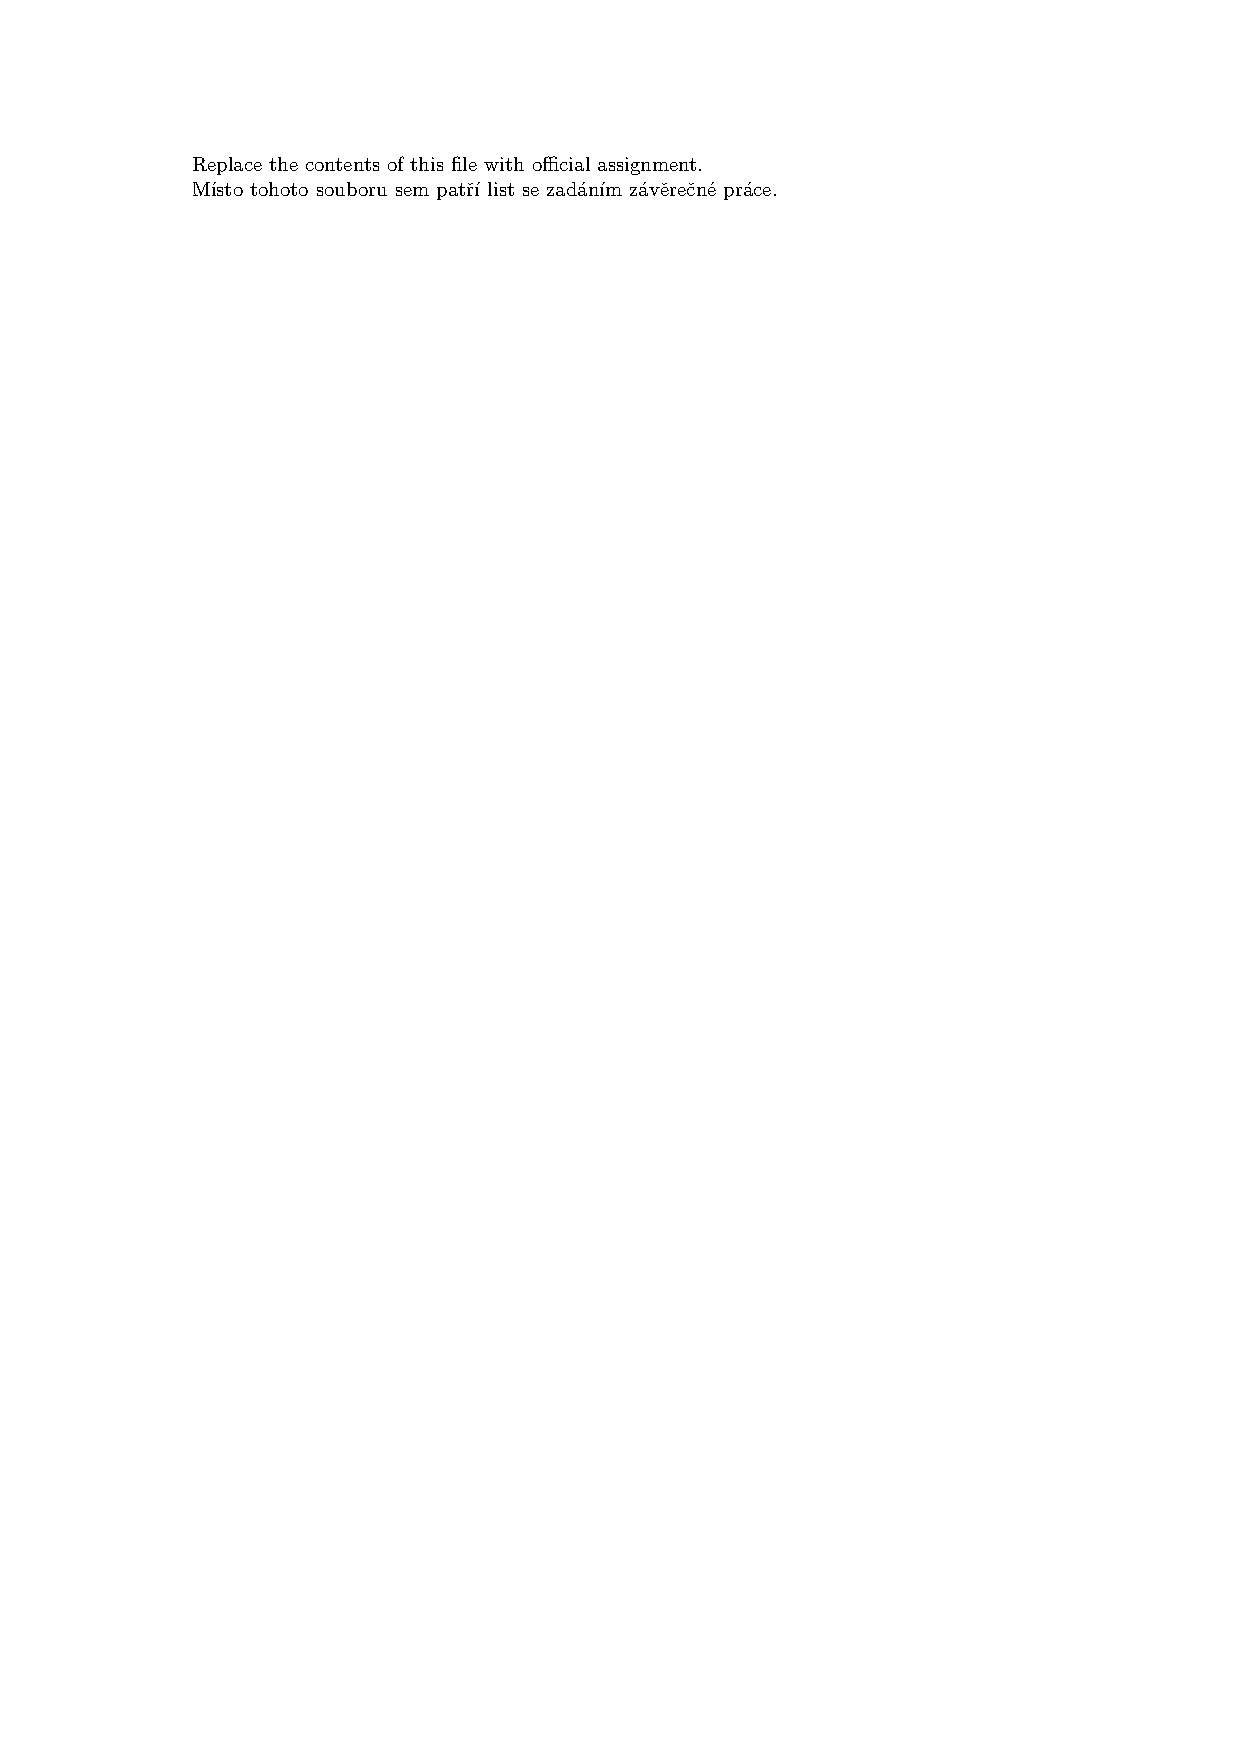
\includepdf[pages={1-}]{assignment-include.pdf} % replace that file with your thesis assignment provided by study office

\thispagestyle{empty}\cleardoublepage\maketitle % do not remove these three commands

\imprintpage % do not remove this command

\tableofcontents % do not remove this command
%%%%%%%%%%%%%%%%%%%%%%
% list of other contents: figures, tables, code listings, algorithms, etc.
% add/remove commands accordingly
%%%%%%%%%%%%%%%%%%%%%%
\listoffigures % list of figures
\begingroup
\let\clearpage\relax
\listoftables % list of tables
\lstlistoflistings % list of source code listings generated by the listings package
% \listoflistings % list of source code listings generated by the minted package
\endgroup
%%%%%%%%%%%%%%%%%%%%%%
% list of other contents END
%%%%%%%%%%%%%%%%%%%%%%

%%%%%%%%%%%%%%%%%%%
% ACKNOWLEDGMENT
% FILL IN / MODIFY
% This is a place to thank people for helping you. It is common to thank your supervisor.
%%%%%%%%%%%%%%%%%%%
\begin{acknowledgmentpage}
	Chtěl bych poděkovat především sit amet, consectetuer adipiscing elit. Curabitur sagittis hendrerit ante. Class aptent taciti sociosqu ad litora torquent per conubia nostra, per inceptos hymenaeos. Cras pede libero, dapibus nec, pretium sit amet, tempor quis. Sed vel lectus. Donec odio tempus molestie, porttitor ut, iaculis quis, sem. Suspendisse sagittis ultrices augue.
\end{acknowledgmentpage} 
%%%%%%%%%%%%%%%%%%%
% ACKNOWLEDGMENT END
%%%%%%%%%%%%%%%%%%%


%%%%%%%%%%%%%%%%%%%
% DECLARATION
% FILL IN / MODIFY
%%%%%%%%%%%%%%%%%%%
% INSTRUCTIONS
% ENG: choose one of approved texts of the declaration. DO NOT CREATE YOUR OWN. Find the approved texts at https://courses.fit.cvut.cz/SFE/download/index.html#_documents (document Declaration for FT in English)
% CZE/SLO: Vyberte jedno z fakultou schvalenych prohlaseni. NEVKLADEJTE VLASTNI TEXT. Schvalena prohlaseni najdete zde: https://courses.fit.cvut.cz/SZZ/dokumenty/index.html#_dokumenty (prohlášení do ZP)
\begin{declarationpage}
FILL IN ACCORDING TO THE INSTRUCTIONS. VYPLŇTE V SOULADU S POKYNY. Lorem ipsum dolor sit amet, consectetuer adipiscing elit. Curabitur sagittis hendrerit ante. Class aptent taciti sociosqu ad litora torquent per conubia nostra, per inceptos hymenaeos. Cras pede libero, dapibus nec, pretium sit amet, tempor quis. Sed vel lectus. Donec odio tempus molestie, porttitor ut, iaculis quis, sem. Suspendisse sagittis ultrices augue. Donec ipsum massa, ullamcorper in, auctor et, scelerisque sed, est. In sem justo, commodo ut, suscipit at, pharetra vitae, orci. Pellentesque pretium lectus id turpis.

Lorem ipsum dolor sit amet, consectetuer adipiscing elit. Curabitur sagittis hendrerit ante. Class aptent taciti sociosqu ad litora torquent per conubia nostra, per inceptos hymenaeos. Cras pede libero, dapibus nec, pretium sit amet, tempor quis. Sed vel lectus. Donec odio tempus molestie, porttitor ut, iaculis quis, sem. Suspendisse sagittis ultrices augue. Donec ipsum massa, ullamcorper in, auctor et, scelerisque sed, est. In sem justo, commodo ut, suscipit at, pharetra vitae, orci. Pellentesque pretium lectus id turpis.
\end{declarationpage}
%%%%%%%%%%%%%%%%%%%
% DECLARATION END
%%%%%%%%%%%%%%%%%%%

\printabstractpage % do not remove this command

%%%%%%%%%%%%%%%%%%%
% SUMMARY
% FILL IN / MODIFY
% OR REMOVE ENTIRELY (upon agreement with your supervisor)
% (appropriate to remove in most theses)
%%%%%%%%%%%%%%%%%%%
% \begin{summarypage}
% \section*{Summary section}
% 
% \lipsum[1][1-8]
% 
% \section*{Summary section}
% 
% \lipsum[2][1-6]
% 
% \section*{Summary section}
% 
% \lipsum[3]
% 
% \section*{Summary section}
% 
% \lipsum[2]
% 
% \section*{Summary section}
% 
% \lipsum[1][1-8] Lorem lorem lorem.
% \end{summarypage}
%%%%%%%%%%%%%%%%%%%
% SUMMARY END
%%%%%%%%%%%%%%%%%%%

%%%%%%%%%%%%%%%%%%%
% ABBREVIATIONS
% FILL IN / MODIFY
% OR REMOVE ENTIRELY
% List the abbreviations in lexicography order.
%%%%%%%%%%%%%%%%%%%
\chapter{Seznam zkratek}
	
\begin{tabular}{rl}
DFA & Deterministic Finite Automaton\\
FA & Finite Automaton\\
LPS & Labelled Prüfer Sequence\\
NFA & Nondeterministic Finite Automaton\\
NPS & Numbered Prüfer Sequence\\
XML & Extensible Markup Language\\
XPath & XML Path Language\\
XSLT & eXtensible Stylesheet Language Transformations\\
W3C & World Wide Web Consortium
\end{tabular}
%%%%%%%%%%%%%%%%%%%
% ABBREVIATIONS END
%%%%%%%%%%%%%%%%%%%

\mainmatter\mainmatterinit % do not remove these two commands

%%%%%%%%%%%%%%%%%%%
% THE THESIS
% MODIFY ANYTHING BELOW THIS LINE
%%%%%%%%%%%%%%%%%%%

% Do not forget to include Introduction
%---------------------------------------------------------------
% \chapter{Introduction}
% uncomment the following line to create an unnumbered chapter
\chapter*{Introduction}\addcontentsline{toc}{chapter}{Introduction}\markboth{Introduction}{Introduction}
%---------------------------------------------------------------
\setcounter{page}{1}

% The following environment can be used as a mini-introduction for a chapter. Use that any way it pleases you (or comment


%---------------------------------------------------------------
\section{Podkapitola}
%---------------------------------------------------------------


%---------------------------------------------------------------
\chapter{Průzkum stávajících řešení}
%---------------------------------------------------------------

%---------------------------------------------------------------
\section{Závěrečné práce studentů FIT ČVUT na podobné téma}
%---------------------------------------------------------------

\subsection{Bc. Jakub Vejr - Webové prostředí pro správu a konfiguraci IoT projektů}

V této diplmové práci autor popisuje jím vytvořenou aplikaci, která má za úkol zaznamenávat příchozí data ze senzorů, zpracovávat je, a tyto data a trendy z nich vycházející poté zobrazovat pomocí webového rozhraní. Autor si vybral jako hlavní platformu projektu jazyk JavaScript, přesněji řečeno Node.js a frameworku Express. Jednotlivá zařízení komunikují s backendovou částí projektu pomocí REST API, která poté data rozklíčuje z příchozích souborů a pomocí databáze MongoDB je uchovává. Uživatelé této aplikace jsou rozděleni na správce s možností přidávat uživatele i IOT zařízení, a běžné uživatele, kteří pracují jen s omezenou množinou dat. Frontendová část aplikace je napsaná pomocí Next.js a knihovny React. Aplikace tedy funguje především směrem od zařízení k cílovému uživateli, který nemá možnost své IOT zařízení ovládat. 

\subsection{Bc. Jan Prášil - Webová aplikace pro sběr a zpracování dat IoT}

Diplomová práce pana Prášila popisuje a vytváří aplikaci, která má být na frontendové straně de facto upravenou a personalizovanou úpravou JavaScript knihovny Grafana, která se používá k analýze a zobrazování nejrůznějších typů dat s možností notifikace uživatelů, na backendové straně se poté využívá Node.JS, který provozuje REST API, přes který se poté připojuje klientské rozhraní. Backend také komunikuje se službou Microsoft SharePoint Server 2013, což bylo jedním z požadavků při zadávání této práce. Jedná se o podnikovou aplikaci dělanou na míru, díky které mohou uživatelé s pravomocemi v aplikaci rozdělenými dle typu jejich účtu provádět správu IOT zařízení, nebo si zobrazovat údaje z nich získané. Tato aplikace také funguje spíše jako jednosměrný kanál informací.

\subsection{Martin Skalický - IoT platforma s webovým rozhraním}



%---------------------------------------------------------------
\section{Existující řešení}
%---------------------------------------------------------------

V dnešní době najdeme na trhu nepřeberné množství produktů, které nám umožní interakci s IOT zařízeními. Pro širší veřejnost jsou pravděpodobně známější produkty od velkých nadnárodních společností, které se nespecializují výhradně na tvorbu IOT platforem, ale tyto produkty vytváří spíše jako přesah svých dalších služeb, jako je například Google Home od společnosti Google, nebo SmartThings od společnosti Samsung. Ty jsou známě především díky skvělé integraci těchto platforem přímo do operačních systémů těch zařízení, které jsou vyráběny právě v koprodukci těchto globálních gigantů. Tento trend ale nepozorujeme pouze u firem populárních na západní hemisféře, stejnou cestu například zvolila i společnost Xiaomi a její aplikace na správu a ovládání IOT zařízení pojmenovaná Xiaomi Home.

Do další skupiny můžeme zařadit produkty, které jsou vyvíjeny úspěšnými společnostmi, které se speializují na výrobu přímo IOT zařízeních jako takových, a pro snadné propojení svých zařízení mezi sebou vytvořili svou vlastní IOT platformu. Takovými společnostmi jsou například Philips a její Philips Hue, používaný primárně pro ovládání všech typů domácího osvětlení od tohoto výrobce, TP-LINK se svým nově vzniklou řadou produktů Tapo, EVOLVEO a aplikace na správu kamer EVOLVEO CAM.

V průběhu let se ale ukázalo, že omezovat svá zařízení pouze na jedinou, a často totožnou společností produkovanou, možnost, jak je může jejich uživatel ovládat, je z byznisového hlediska nečekaně kontraproduktivní, jelikož pouze minimum zákazníků používá všechna chytrá zařízení vyrobená pouze jednou firmou. Jednotlivé firmy mají totiž často nerovnoměrnou kvalitu i kvantitu možností napříč jednotlivými typy IOT zařízení a proto je pro zákazníka nejpohodlnější koupit si různé výrobky od různých firem. Proto se na trhu staly populárními zařízení podporující několik, a často i konkurenčních, ovládacích aplikací.

V této době začly vznikat i projekty společností i jednotlivců, které cílí pouze na tvorbu ovládačího softwaru pro co nejvíce typů IOT zařízení napříč výrobci, ale samy zařízení jako takové nevyrábí. Díky oblíbenosti a řádově menším nákladům je těchto projektů v dnešní době dostupných desítky až stovky. Některé z nich jsou dokonce tak populární, že sami výrobci inzerují své IOT zařízení s informací, že podporují ovládaní těmito prostředky. Jejich nevýhodou oproti řešením popsaných výše jsou ale často poplatky za použití, jelikož narozdíl od společností, které svůj výdělek získají z prodeje hardwaru a ovládací software často přikládají zdarma, společnosti bez hardwaru musí získávat peníze na vývoj a údržbu těchto produktů jinými způsoby, a to často právě prodejem přístupu k těmto ovladačům, nebo zpoplatněním některých jejich služeb.

Poslední skupinou jsou opensource projekty, tedy projekty, které mají veřejně dostupný zdrojový kód. Tyto produkty se vyznačují tím, že za nimi často stojí dobrovolnická komunita nadšenců, kteří často projekt vytváří ve svém volném čase, většinou jsou také tyto produkty kompletně zdarma, nebo maximálně s placenými vylepšeními. Mají však ale také své nevýhody, často nejsou tak uživatelsky přívětivé jako placené, komerčně vytvářené alternativy. I přes občasnou menší funkcionalitu, způsobenou například nedostatkem veřejně dostupné dokumentace k určitým zařízením, se takové projekty stávají stále oblíbenějšími.

%---------------------------------------------------------------
\section{Funkční řešení}
%---------------------------------------------------------------

V této části je popsáno několik známých a rozšířených řešení. Ty jsou poté porovnány na základě jejich vlastností.

\subsection{Particle}

Projekt Particle vznikl v roce 2013 v americkém městě San Francisco. Zakladatel firmy Particle, tehdy ještě pojmenované Spark, prý s tímto IOT projektem začal, když chtěl vyrobit svému hluchému otci světlo, které by zablikalo a upozornilo ho, kdykoliv by mu na telefon přišlo oznámení. Brzy na to tedy vyrobil první IOT zařízení a ovládací software k němu. V následujících letech se firma soustředila především na vývoj programovatelných řídících obvodů, které uživatel připojí ke svému spotřebiči nebo senzoru, který chce mít možnost ovládat jako IOT zařízení. Tento řídící obvod se poté, v závislosti na konkrétním provedení obvodu, pomocí technologií jako WiFi nebo mobilních sítí připojí k řídícímu cloudu, vydanému a provozovanému téže společností. Cloud má poté standardizované rozhraní pro propojení jak se známými a na trhu dostupnými nástroji pro správu IOT zařízení, tak i pro propojení s na míru zákazníkem vyrobenou aplikací. 

Particle je řešení především pro začínající firmy, které mají zařízení, které dosud není možné propojit s žádnou stávající (a to ani vlastní) chytrou platformou. Particle takovým zařízením zprostředkuje to, co odlišuje chytré IOT zařízení od běžného zařízení a zbytek už nechává na implementaci zákazníkem. V té se mu ale alespoň snaží asistovat nabídkou rozsáhlé dokumentace několika API, kterými s Particle cloudem můžou aplikace zákazníka komunikovat, ale také v neposlední řadě i vlastním programovacím prostředím založeným na produktu firmy Microsoft zvaném Visual Studio. Dále také nabízí doplňkové služby jako je nepřetržitý monitoring dostupnosti zařízení a případný servis, který ať už vzdáleně, nebo přímo na místě zkusí vyřešit případný problém s konektivitou zařízení.

Produkty Particle jsou dostupné v několika balíčkách, od nejlevnějšího balíčku "Free", který je zadarmo, nabízí až 100 zařízení a na nich až 100000 vykonaných operací, a je doporučován pro seznámení se s touto platformou, přes balíček "Plus", který nabízí stejný počet zařízení, ale až 5 milionů vykonaných operací, až po balíčky "Professional" a "Enterprise", které předem nejsou naceněné a zákazník si je může vyjednat dle jeho specifických požadavků.  

Produkty Particle jsou využívány například společnostmi Zoomo nebo Olulo (výroba elektrických vozidel), Watsco a Intellihot (HVAC systémy), Qube (kontrola emisí), nebo Dentalez a Amper (obecný monitoring industriálních nástrojů).

\subsection{ThingsBoard}

ThingsBoard je souhrnný název pro skupinu produktů založenou v roce 2016, který svým zákazníkům nabízí mnoho funkcí týkajících se správy vlastních IOT zařízení. Primárním a nejpopulárnějším produktem je stejnojmenná IOT platforma ThingsBoard. Ta slibuje jednoduchý vývoj, správu a růst IOT projektů svých zákazníků, kterého se snaží docílit pomocí několika modulů. Prvním takovým je modul komunikace s IOT zařízeními, který podporuje mnoho komunikačních bran, ať už známější jako HTTP, MQTT, CoAP nebo SNMP, tak i méně známé OPC-UA, modbus a další. Dalším je modul výpočetní, nazývaný ThingsBoard Core, který je napsaný v jazyce Java a má na starost zprostředkovat REST komunikaci s webovým rozhraním, komunikaci s databází, s jednotlivými IOT zařízeními a také zpracování příchozích i odchozích zpráv řetězci pravidel, v originále nazývaných ThingsBoard Rule Chains, které výpočetnímu modulu přikazují jednotlivé kroky, které musí být provedeny, jako je ověření telemetrických dat ze zařízení, tvorba upozornění v závislosti na dostupnosti zařízení, tvorba REST volání do externích systémů, kontrola parametru příchozí zprávy a mnoho dalších. K uchování persistentních dat nabízí ThingsBoard propojení s SQL databází, PostgreSQL, i noSQL databází, Cassandra. Posledním, předem zmíněným modulem je ThingsBoard Web UI, který zajištuje možnost nastavovat všechny ostatní moduly a jednotlivé části, od komunikace s IOT zařízením po tvorbu komplexních řetězců pravidel.

ThingsBoard IOT platforma nabízí několik typů předplatného. Prvním je takzvaná Community Edition, která je kompletně zdarma a její zdrojové kódy jsou dokonce opensource. Toto předplatné nám umožňuje přidat neomezený počet zařízení. Pokud ale zaplatíme za jakoukoliv z placených edic, u kterých si navíc můžeme vybrat, zda chceme využít hosting od společnosti ThingsBoard, nebo zda chceme pouze možnost používat jejich služby, ale hosting si zařídíme sami, získáme výhody jako je emailová podpora, whitelabeling, neboli možnost provozovat syto služby pod svým názvem a logem, a u nejdražších edic dokonce získáme i 10 hodin konzultací s expertem nebo dokonce několik školení pro naše zaměstnance. Máme také možnost si koupit služby v balíčku Trendz Analytics, pomocí kterých můžeme dále data získaná z našich zařízení analyzovat, detekovat anomálie, ale i predikovat možné hodnoty. Dále nám také nabízí více možností vizualizace dat. Posledním produktem nabízeným na stránkách projekty ThingsBoard je ThingsBoard Edge, který slouží k filtrování velkého množství dat přicházejících od IOT zařízení do ekosystému ThingsBoard, které přinese větší přehlednost a rychlost běhu.

\subsection{thethings.iO}

thethings.iO je projekt vyvíjený firmou Diprotech sídlící ve španělské Barceloně. Tento projekt nabízí nástoje pro připojení, správu a ovládání chytřých zařízení, případně také na získávání, uchovávání a analyzování dat z nich. K tomu slouží webové rozhraní, které komunikuje s hlavní aplikací, napojenou na jednotlivá IOT zařízení. thethings.iO nabízí několik balíčků služeb, u kterých s narůstající cenou narůstá počet funkcionalit a možnosti upravit si produkty na míru. Tato společnost nenabízí žádný balíček zdarma, nejlevnější začíná s cenou na 25€, za kterou může jediný uživatel připojit až 10 zařízení. V dražších balíčcích ale může bých uživatelů více, narůstá také počet možných připojených zařízení a přidávají se výhody jako telefonická podpora nebo možnost změnit logo a jméno zobrazované na ovládací webové stránce z loga thethings.iO na jakékoliv jiné. V případě koupě nejdražších balíčků pak do určité míry mohou zákazníci vydávat tyto produkty za své a budí tak větší pocit profesionality. thethings.iO se od ostatních pdobných produktů od jiných výrobců odlišuje například důrazem na zabezpečení dat konečných klientů používajících webové rozhraní. Nabízí sadu funkcionalit pojmenovanou Retailer Blinder Tool, pomocí kterých lze vytvářet jednotlivé účty pro jednotlivé klienty, které mají různé rozsahy pravomocí a mohou například spravovat pouze určitá zařízení. 

thethings.iO také nabízí možnost data přijatá z jednotlivých zařízení nejprve zpracovat, předtím, než je uloží nebo zobrazí klientům, a toto zpracování lze ve webovém rozhraní nadefinovat pomocí takzvaného Cloud Code. To je systém složený z mnoha předdefinovaných spouštěčů, které reagují na příchozí signály nebo příchodí data, a funkcí psaných v JavaScript jazyku, které si může zákazník sám nadefinovat. Tyto funkce potom mohou být dle libosti kombinovány a dokonce spouštěny externě, jelikož každá z nich má veřejně dostupnou URL. Tyto funkce mohou být také spouštěny automaticky časovačem.

IOT zařízení se systémem thethings.iO můžou komunikovat pomocí několika protokolů, jmenovitě HTTP, MQTT a Websockets. Naopak místo frontendové webové aplikace mohou zákazníci používat předem definovaný REST API, nicméně ten neobsahuje veškeré funkcionality webového rozhraní. Dalšímy podporovanými výstupy ze systému je možnost dostávat informační SMS nebo telefonní hovory díky propojením se společností Twilio, dostávat informační emaily od společnosti SendGrid, nebo také zprávy na sociální sítě WhatsApp a Telegram, přičemž na druhém jmenovaném je možnost propojení s na míru vytvořeným chatbotem. Klasickými dostupnými integračními kanály jsou pak Google Home Assistant a Amazon Alexa.

Projekt je vyvíjen přednostně pro zákazníka, který je společností menší nebo střední velikosti, která dodává nebo pronajímá IOT zařízení a s nimi spojené služby jiným, větším, pravděpodobně netechnicky zaměřeným firmám. Typickým příkladem by byl imaginární podnikatel Novotný, který by se svou firmou čítající jeho a dva kolegy zajišťoval chytré čidla do mrazících boxů a automatické rolety do vchodových dveří pro místní pobočky supermarketů, například Albert, Tesco a Billu. Díky produktům thethings.iO by se pak mohli zaměstnanci těchto supermarketů každý připojit na stránku novotny.cz, kde by po přihlášení každý viděl a ovládal pouze svá zařízení a data z nich. Firma pana Nováka by přitom ale musela jen koupit a namontovat samotná zařízení a poté už je jen připojit do stávajícího řešení od thethings.iO. 

\subsection{openHAB}

openHAB je opensource projekt spravovaný nonprofitovou organizací openHAB Foundation e.V. Umožňuje propojení několika ze seznamu zhruba 2000 podporovaných IOT zařízení s řídícím programem, který disponuje vlastním konfigurovatelným webovým rozhraním. Narozdíl od mnoha jiných konkurenčních řešení inzeruje primárně možnost stáhnout si svůj vlastní backendový server a spouštět ho na vlastním počítači, zatímco většina ostatních firem cílí na pronajímání přístupu k jimi hostovaným cloudovým službám. Tento server je k dispozici na mnoho platformách, například Windows, Linux, macOS, nechybí ale ani Respberry Pi, Docker nebo Synology. Uživatelé zároveň mohou využít jak přístupu k serveru pomocí webového rozhraní, tak i pomocí bezplatné aplikace pro Android i iOS. 

Díky tomu, že se na vývoji podílí velké množství programátorů, a každý z nich k projektu přidává kompatibilitu s jinými typy zařízení a platformami, disponuje openHAB oproti svým konkurentům větším výběrem a to v mnoha ohledech. Kromě klasických výrobců chytrých zařízení, kteří mají své komunikační protokoly zveřejněné a díky své popularitě je můžeme připojit téměř k jakémukoliv dostupnému IOT systému, openHAB nabízí propojení zařízení netradičnějších, jako jsou zařízení od značky Epson, Chromecast, Bosch, Bose, AndroidTV, Renault, Spotify, ale zvládne dokonce připojit jako IOT zařízení i běžící multiplayer server populární hry Minecraft.

Pokud není uživatel fanouškem webových nebo mobilních aplikací pro ovládání tohoto systému, openHAB podporuje několik způsobů a aplikací, díky kterým lze celý systém jako takový propojit s jiným konkurenčním IOT systémem a používat některé jeko funkcionality. Stačí, aby danou metodu komunikace a propojení podporoval i tento propojovaný systém. Příkladem těchto možných integrací jsou například Metrics service, openHAB Cloud Connector, openHAB Hue Emulation a další.

Velkou nabídku alternativ nabízí openHAB i co se týče zpracování a uložení dat, které získáme ze svých zařízení. Pro zpracovávání můžeme využít jakýkoliv předem napsaný plugin ze široké konumitní knihovny, nebo si plugin můžeme napsat vlastní, a to v jazycích jako Groovy, JavaScript, JRuby nebo Jython. Pro upládání persistentních dat lze potom použít mongoDB, InfluxDB, JDBC, MapDB a další. Nativně implementované jsou ale i menší funkce, které ale uživateli při správném použití mohou ušetřit mnoho času, jako je třeba podpora XPath pro zpracovávání dat z XML souborů. V neposlední řadě také podporuje projekt možnost komunikace pomocí speech-to-text a opačnou text-to-speech.

openHAB má v nabídce možnost využít hostovaný cloudový systém, nicméně sám zřizovatel varuje, že tento systém nemusí být vždy dostupný a měl by být používaný spíše jako demonstrace nebo pro vyzkoušení a ověření funkcionality předtím, než se budoucí zákazník pustí do instalace a zprovozňování tohoto systému, který v tomto ohledu může být o něco technicky náročnější než konkurenční alternativy.

\subsection{Home Assistant}

Home Assistant je dalším z mnoha opensource projektů vytvořených pro správu a ovládání IOT zařízení. Hlavní části projektu jsou psané v jazyce Python. Tato část se poté spouští na lokálním zařízení, není tedy k dispozici možnost ani placeného cloudového řešení. Případ, že by zákazník neměl žádné zařízení, na kterém by mohl tento program spustit, se komunita tvořící Home Assistant rozhodla vyřešit jinak - a to tak, že na webových stránkách projektu nabízí ke koupi předinstalovaná zařízení na bázi Raspberry Pi, které si zákazník objedná a zařízení je v podstatě plug-and-play. Další možností je poté spouštět program v kontejneru pro Docker na svém osobním počítači. Docker řešení má výhodu nezávislosti na operačním systému daného počítače, ale tento způsob používání systému nepodporuje veškeré funkcionality, například nemá možnost být na dálku zresetován do předem zálohovaného stavu.

Home Assistant je řešení, které spoléhá na větší uživatelské schopnosti v oblasti IT, než vyžaduje běžná konkurence. Například kompletní nastavení samotného backendu není kompletně přístupné pomocí GUI, ale uživatel musí nejprve nastavit hodnoty přímo do konfiguračních souborů. Ty jsou sice v uživatelsky přívětivém formátu YAML, nicméně i přes to se jedná o uživatelsky náročnější proces. 

Home Assitant umožňuje takzvanou automatizaci zařízení, kde si uživatel může nadefinovat chování zařízení a procesy, které mají být spuštěny, v případě, že nastane popsaná událost. Tato automatizace sice je uživatelsky přívětivá, především díky přítomnosti GUI, které zákazníka kompletně provede tvorbou takových pravidel, nevýhodou ale je, že je zákazník omezen pouze na nízký počet předdefinovaných akcí a 
pokud chce automatizovat jinou, není žádný jednoduchý způsob, jak toho docílit. Home Assistant také nabízí možnost použití a pouhé upravení jistých vzorů, v originále zvaných Automation Blueprints, které vytvořili ostatní uživatelé, takže pokud nechce zákazník vytvářet vlastní pravidla, stačí si vybrat a poté importovat správný vzor z komunitního fóra této aplikace.

Automatizovat se dá také pomocí skriptů, které jsou však pouze zapsanými pravidly, které bychom mohli vytvořit pomocí výše popsaného GUI, v jazyce YAML. K dispozici jsou příkazy pro porovnání dvou proměnných, možnost poslat příkaz určitému zařízení, počkat na předem popsaný jev a opakování několika příkazů v cyklu. Oproti konkurenčním implementacím skriptovaných pravidel je u Home Assistent projektu menší flexibilita a možnost kreativity.

Home Assistant nabízí také nativní podporu ovládání pomocí hlasových příkazů, a po pomocí modulu Assist. Ten je součástí jak webového rozhraní, tak i mobilních aplikací, kterými lze celou chytrou domácnost ovládat. Celá domácnost pak může mít definované hlasové příkazy ve známých asistentech jako je Amazon Alexa, Siri nebo Google Assistant, pomocí kterých může uživatel také interagovat se zařízeními, pokud nechce nebo nemůže využít hlasové ovládání vytvořené přímo vývojáři tohoto projektu.

Webové rozhraní, stvořené pro ovládání zařízení, nabízí dlaždicový vzhled stránky, přičemž dlaždice si každý uživatel může sám rozmístit, přidat a upravit. K dispozici je 29 typů základních dlaždic, od jednoduchých prvků, které pouze ukazují teplotu z čidel, až po dlaždici zobrazující detailní mapu ovládané domácnosti a lokace jednotlivých spotřebičů na ní. Pokud by ani jeden z těchto typů dlaždice nevyhovoval, je také možnost přidat dlaždice vytvořené komunitou. Ty můžeme, stejně jako celý zdrojový kód tohoto projektu, najít na GitLabu společnosti.

Podporovaná zařízení

\subsection{ThingSpeak}

ThingSpeak je opensource projekt od společnosti MathWorks, americké firmy specializující se na tvorbu matematických vizualizačních a výpočetních programů, jako je například MATLAB nebo Simulink. Ačkoliv je tato společnost na trhu už přes 35 let, projekt ThingSpeak vznikl až v roce 2010. Zdrojový kód aplikace je psaný v jazyce Ruby. Výhodou tohoto projektu je hluboká možnost propojení IOT zařízení s ostatními produkty od tohoto vydavatele, především s aplikací MATLAB. Díky tomu lze tuto platformu využívat k případům, kdy je potřeba data zpracovávat výkonějším strojem, než je běžný IOT hub, jako je například analýza živého videa z bezpečnostní IP kamery.

ThingSpeak bohužel naopak nepodporuje velké množství protokolů pro komunikaci s IOT zařízeními, data lze dodávat pouze pomocí REST API, nebo pomocí MQTT. U každého příchozího kanálu dat poté můžeme definovat která data se můžou zobrazovat jako veřejná a která jsou pouze pro soukromé účely, díky čemuž se poté na hlavní stránce celého projektu můžeme inspirovat projekty jiných uživatelů, nebo dokonce jejich produkty využívat v běžném životě, jelikož jsou v nabídce například i podrobná data z mnoha meteostanic po celém světě. 

Pomocí modulu MATLAB Analysis můžeme nechat ThingSpeak komunikovat s kódem v aplikaci MATLAB a tam data transformovat, agregovat, používat je v pokrořilých matematických operacích a poté je pomocí modulu MATLAB Visualization tyto data prezentovat v různých typech grafů, tabulek a dalších médiích. Pomocí aktivovatelných rozšíření pro aplikaci MATLAB, jako jsou ThingTweet, TimeControl, TalkBack, React nebo ThingHTTP můžeme implementovat běžně očekávatelné funkcionality konkurenčních IOT hubů, jako je možnost provádět příkazy v závislosti na datech, na čase, nebo na výsledku jiných operací. Také lze posílat příkazy nebo jiná data zpět k IOT zařízení. Zároveň si můžeme nechat zasílat oznámení pomocí propojení se sociální sítí Twittter.

Většina těchto funkcí je omezena pouze pro držitele platné licence, nicméně ThingSpeak nabízí jak licence pro studenty, tak i pro akademické nebo domácí použití, přičemž ty poté za splnění určitých podmínek a omezení mohou být i zdarma. Nabízena je ale také i komerční licence pro industriální objemy dat a zařízení.

V praxi se s aplikací ThingSpeak jakožto produktem pro business použití můžeme potkat například u projektů na efektivní chytré zemědělství, kde zemědělci získávají data o složení půdy, vlhkosti, teplotě a dalších faktorech, aby zvládli lépe plánovat své kroky, u projektů na monitorování elektrické energie, její spotřeby, trendů, ale také například při výrobě energie v menších elektrárnách. V neposlední řadě je také platforma ThingSpeak používána k zaznamenávání kvality ovzduší a ostatních měřitelných hodnot o životním prostředí. Naopak u jednotlivců, kteří chtějí vyrábět malé domácí sítě můžeme narazit na statistiky o jejich chytré domácí meteostanici, nebo třeba o hodnotách z čerpadla a filtrace jejich zahradních bazénů.

\subsection{Blynk}

Blynk je projekt založený Pavlem Bayborodinem v roce 2014, který svým uživatelům umožňuje připojit zařízení svá standardizovaná IOT zařízení k na míru vytvořeným aplikacím, které tato společnost také dodává. Zakladatel tohoto projektu je bývalý tvůrce uživatelských rozhraní a expert v oblasti UI/UX, a pravděpodobně proto se i celá firma zaobírá především jednoduchostí ovládání neznalejším uživatelem a upřednostňuje grafické ovládací prvky před větší univerzálností, které by šlo jednodušeji docílit při používání programovacích jazyků a jiných, techničtějších přístupů k ovládání a nastavování produktů. Blynk jako první v oboru nabídl uživatelům možnost vytvořit si vlastní aplikaci čistě z předem vytvořených modulů, které si jen uživatel předem naskládá do požadovaného rozvržení a aplikace se poté sama vytvoří dle jeho představ, a to dokonce v prostředí webového prohlížeče, bez nutnosti instalace jakéhokoliv běžně používaného programu pro vývoj aplikací. Nevýhodou takového řešení je ale jednotvárnost, neoriginalita a neflexibilita při tvorbě speciálních, na míru dělaných IOT zařízení, se kterými předem vytvořené ovládací prvky nepočítají.

Projekt Blynk je rozdělen do několika částí nebo podproduktů. Blynk.Console je webová stránka, která má za úkol poskytnout uživatelům možnost nastavovat a přidávat zařízení, o kterých poté umí zobrazovat všechna nasbíraná data a také je lze pomocí této stránky ovládat. Je zde také možnost upravovat a přidávat uživatele, kteří pak mohou jednotlivá zařízení vidět po svém přihlášení, nebo také spravovat celé organizace neboli skupiny uživatelů. 

Blynk.Apps je Android a iOS aplikace, která slouží jako ovládací prvek k předem přednastaveným IOT zařízení. Může být nakonfigurována předem pomocí Blynk.Console, ale i v průběhu používaní, pokud má uživatel přístup do takzvaného produkčního módu. Blynk nabízí dokonce možnost takzvaného whitelabelingu, neboli možnost vydávat aplikaci i na App Store a Google Play pod svým designem, se svým logem a názvem, ale to pouze při zaplacení dražších business plánů.

Dalšími produkty jsou Blynk.Edgent a Blynk.Library, kde název Edgent vznikl kombinací slov Edge a Agent. Blynk.Edgent je knihovna v jazyce C++ připravená pro připojování podporovaných zařízení ke cloudu společnosti Blynk. Vyskytují se zde příkazy jak pro řízení konektivity přes WiFi, mobilní sítě nebo Ethernet, funkce pro přesnost dat mezi zařízením a cloudem, over-the-air aktualizace firmwaru zařízení a další. Blynk.Library je také C++ knihovna, která se ale zaměřuje především na implementaci streamingového protokolu, díky kterému lze navázat oboustrannou komunikaci s nízkou latencí. 

Blynk.Cloud je infrastruktura serverů, ke které se jednotlivé samostatné části řešení, jako je Android aplikace nebo IOT zařízení, připojují. Blynk také nabízí možnost pronájmu jejich serverů pro své vlastní využití. Na těchto serverech nabízí Blynk takzvané microservices, neboli části softwaru, které fungují napříč produkty Blynk a mají specifické speciální funkce, jako je například Blynk.Air pro aktualizace softwaru na IOT zařízení pomocí OTA technologie, Blynk.R specializující se na správu uživatelů, nebo Blynk.Inject, který nabízí možnost registrace zařízení a dalších kroků a procesů s tímto spojených.

Blynk, na rozdíl od svých konkurentů, na svých stránkách nenabízí seznam podporovaných zařízení jako takových, ale seznam podporovaných čipů nebo integrovaných obvodů, které dané zařízení musí obsahovat a používat ke komunikaci. Připojení těchto zařízení je možné pomocí C++ knihoven Blynk.Library, Blynk.Edgent, pomocí specializovaných NCP čipů, nebo přes HTTP API.

Známými firmami využívající technologií Blynk jsou například Dylos nebo Zeptive z oblasti měření kvality ovzduší, Modular Farms Co nebo Fetzer v oblasti zemědělství, výrobce boilerů Raypak nebo Fiedler, firma, která vyrábí sledovací zařízení nejen pro vozidla.
Blynk nabízí řešení zdarma, které je zamýšleno primárně pro účely seznámení se s prostředím a je velmi omezené, poté předplatné Maker, které je zamýšleno pro jednotlivce/rodiny, jelikož je se svou cenou 7 USD rozumným výdajem a umožňuje registraci až dvaceti zařízení, předplatné Pro za 99 USD, které nabízí všechny typy widgetů v aplikaci, až 1000 uživatelů a až 500 zařízení, nebo Enterprise předplatné, které je potřeba pro možnost whitelabelingu mobilní aplikace a dalších funkcí.


%---------------------------------------------------------------
\section{Porovnání}
%---------------------------------------------------------------
 % include `text.tex' from `text/' subdirectory

\appendix\appendixinit % do not remove these two commands

\chapter{Nějaká příloha}


Sem přijde to, co nepatří do hlavní části.
 % include `appendix.tex' from `text/' subdirectory

\backmatter % do not remove this command

\printbibliography % print out the BibLaTeX-generated bibliography list

\chapter{Obsah příloh}
% Concents of the attachment

	\dirtree{%
		.1 readme.txt\DTcomment{stručný popis obsahu média}.
		.1 exe\DTcomment{adresář se spustitelnou formou implementace}.
		.1 src.
		.2 impl\DTcomment{zdrojové kódy implementace}.
		.2 thesis\DTcomment{zdrojová forma práce ve formátu \LaTeX{}}.
		.1 text\DTcomment{text práce}.
		.2 thesis.pdf\DTcomment{text práce ve formátu PDF}.
	}
 % include `medium.tex' from `text/' subdirectory

\end{document}
